\insertmeeting 
	{Tactical T} 
	{09-22-22}
	{Hagerty High School}
	{Jensen, Jorge, Karissa, Laura, Nathan, Robert, Samantha, Tyler}
	{Images/RobotPics/robot.jpg}
	{2:30 - 4:00}
	
\hhscommittee{General}
\noindent\hfil\rule{\textwidth}{.4pt}\hfil
\subsubsection*{Goals}
\begin{itemize}
    \item Assemble the field

\end{itemize} 

\noindent\hfil\rule{\textwidth}{.4pt}\hfil

\subsubsection*{Accomplishments}
We've been waiting a while for our field parts to arrive, and today is finally the day that they have. Today was only spent assembling the field, using the official FTC instructions as our guide. An interesting limitation we came across was that we share our field with our VEX teams, who's game, Spin Up, divides sides of their field into diagonals. As such, the junctions we assembled could only go as far as the ones that laid on that diagonal. This meant we would only have 15/25 junctions in place. While this wasn't much of an issue for assembly, since VEX hadn't put the tape line usually in place on Spin Up fields, so we didn't need to remove anything. However, issues will arise when we start doing programming and driver practice, as we can't practice with the whole field. We're happy to finally have our field in place, but going forward, we need to be weary of potential oversights caused by this limitation, such as our limited ability to practice circuits, and programming autonomous for certain starting positions.

\hhscommittee{Hardware}
\noindent\hfil\rule{\textwidth}{.4pt}\hfil
\subsubsection*{Goals}
\begin{itemize}
    \item Learn how to make parts out of carbon fiber
	\item Create one of the carbon fiber sides with 3D printed molds

\end{itemize} 

\noindent\hfil\rule{\textwidth}{.4pt}\hfil


\subsubsection*{Hardware}
During this meeting, we hoped to make some real progress on our robot design! The first step of making any robot (aside from planning, which we did in our previous meetings and at kick off) is the drivetrain. After finding success in creating our unique tricycle drivetrain from last season, we were eager to test various designs and were very open-minded to any original ideas. 
To start off the process, we tested the drivetrains we had on hand with this season's field to see how the different approaches to moving around the field would fare against the crowded grid of junctions. First up was the drivetrain used by our sister team, 4227 metal morphosis, for last year's game. Being a tank drive, we felt it was a good place to start as it is one of the most basic, yet popular, types of the drivetrain. When driving it around the field, we found that it was quite difficult to maneuver around the poles. Because of its larger size and somewhat clunky steering, we often found our selfs taking much longer to get from one end of the field to the other than we expected. (figure 1)

Next, we planned to test a mecanum drive. Unfortunately, the only one we have was a prototype from the beginning of last season that has since lost a couple of parts and was in need of reassembling. Before the meeting, we planned to rebuild the mecanum drive, but eager to get started with a new design, we thought about the possibility of passing up on testing it entirely. Because the tank drive and mecanum move and function in much the same way, we thought they would both be front runners for what drivetrain we would choose, making it necessary to test both to see which would come out on top. But because the tank drive had performed worse than we expected and because its problems when turning would also effect the mecanum drive, we decided not to waste time fixing it when we already have a good idea of its shortcomings based on testing the tank drive combined with our past experiences with mecanum.

Last but not least was our robot from last year, Scoopie, whose drivetrain is notably different than FTC standards. Throughout the season last year, we talked to a lot of teams, mentors, and judges, and none of them had seen anything like it used in FTC. Instead of turning by varying the speeds of motors on each side of the drivetrain, as a tank and mecanum drives do, the front wheel turns, vectoring the robot in whatever direction it was pointing. This design gave us more control while turning and perfectly suited the arcing path the robot took moving from the warehouse to the shipping hubs. Despite its advantages from last season, we expected it to struggle weaving between the junctions because of its slightly larger turning radius as compared to a tank drive. Upon putting the robot on the field and going for a spin, we found that once again, our expectations were incorrect. The ability of the tricycle drive to maintain its speed around corners (instead of stopping, turning, then moving again, as tank and mecanum drives must do) made it much quicker when moving from one side of the field to another. The larger turning radius turned out to be much less pronounced than we thought, proving to be more than small enough to swiftly move around the junctions. (figure 2)

After testing the drivetrains and considering our options, we sat down as a group to come up with our plan moving forward. Seeing the failure of the tank drive, we quickly ruled it out, leaving us with three main options: mecanum, which provides a small amount more maneuverability than tank, but suffers from many similar problems when turning, tricycle drive, which turns smoothly but may be slightly unstable because of its smaller amount of wheels, and another option entirely, like x-drive, h-drive, or swerve drive, which we were unable to test but have many problems that in almost every case make them poor options for FTC. In the end, we decided to create a mecanum prototype as a backup, while moving forward with a tricycle drive as our main drivetrain. We decided to split the tasks between members, assigning some to work on the backup mecanum drive and others to work on the tricycle drive, hoping to do some more research after breaking up into our selected groups.

 
\begin{figure}[ht]
\centering
\begin{minipage}[b]{.48\textwidth}
  \centering
  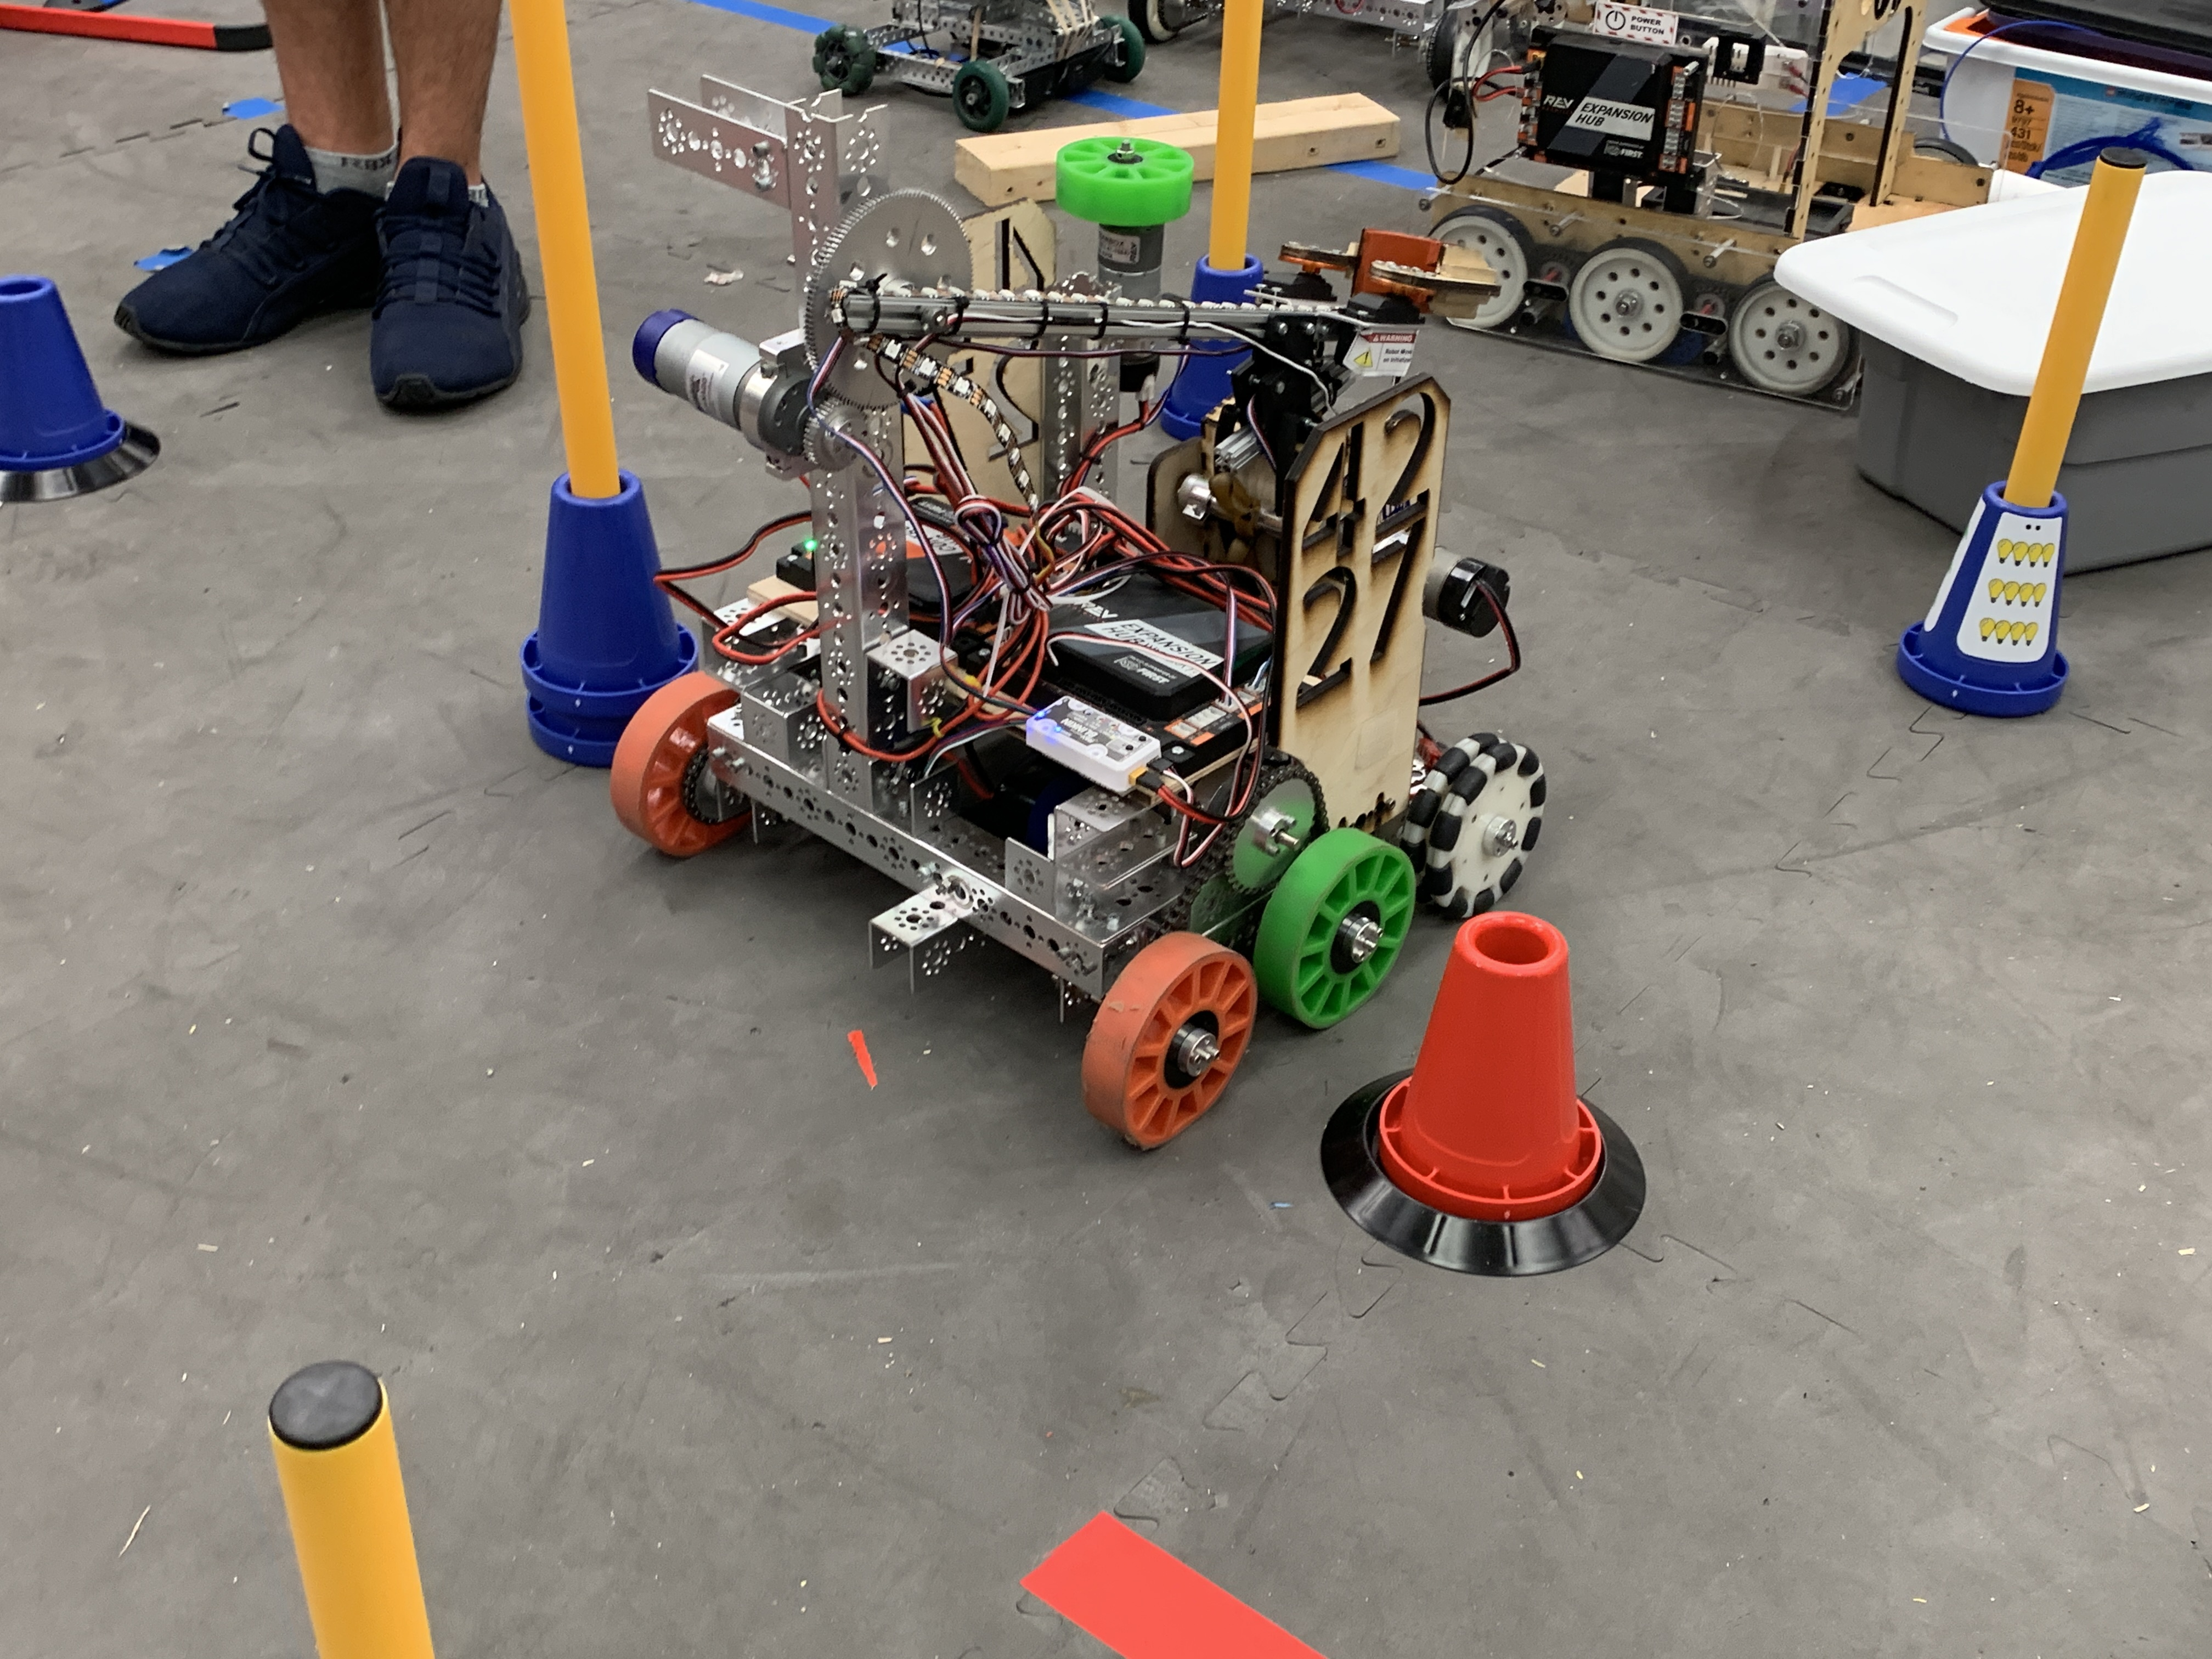
\includegraphics[width=0.95\textwidth]{Meetings/September/09-22-22/9-22-22_Hardware_Figure1.JPG}
  \caption{4227 robot from 2021-2022 season}
  \label{fig:pic1}
\end{minipage}%
\hfill%
\begin{minipage}[b]{.48\textwidth}
  \centering
  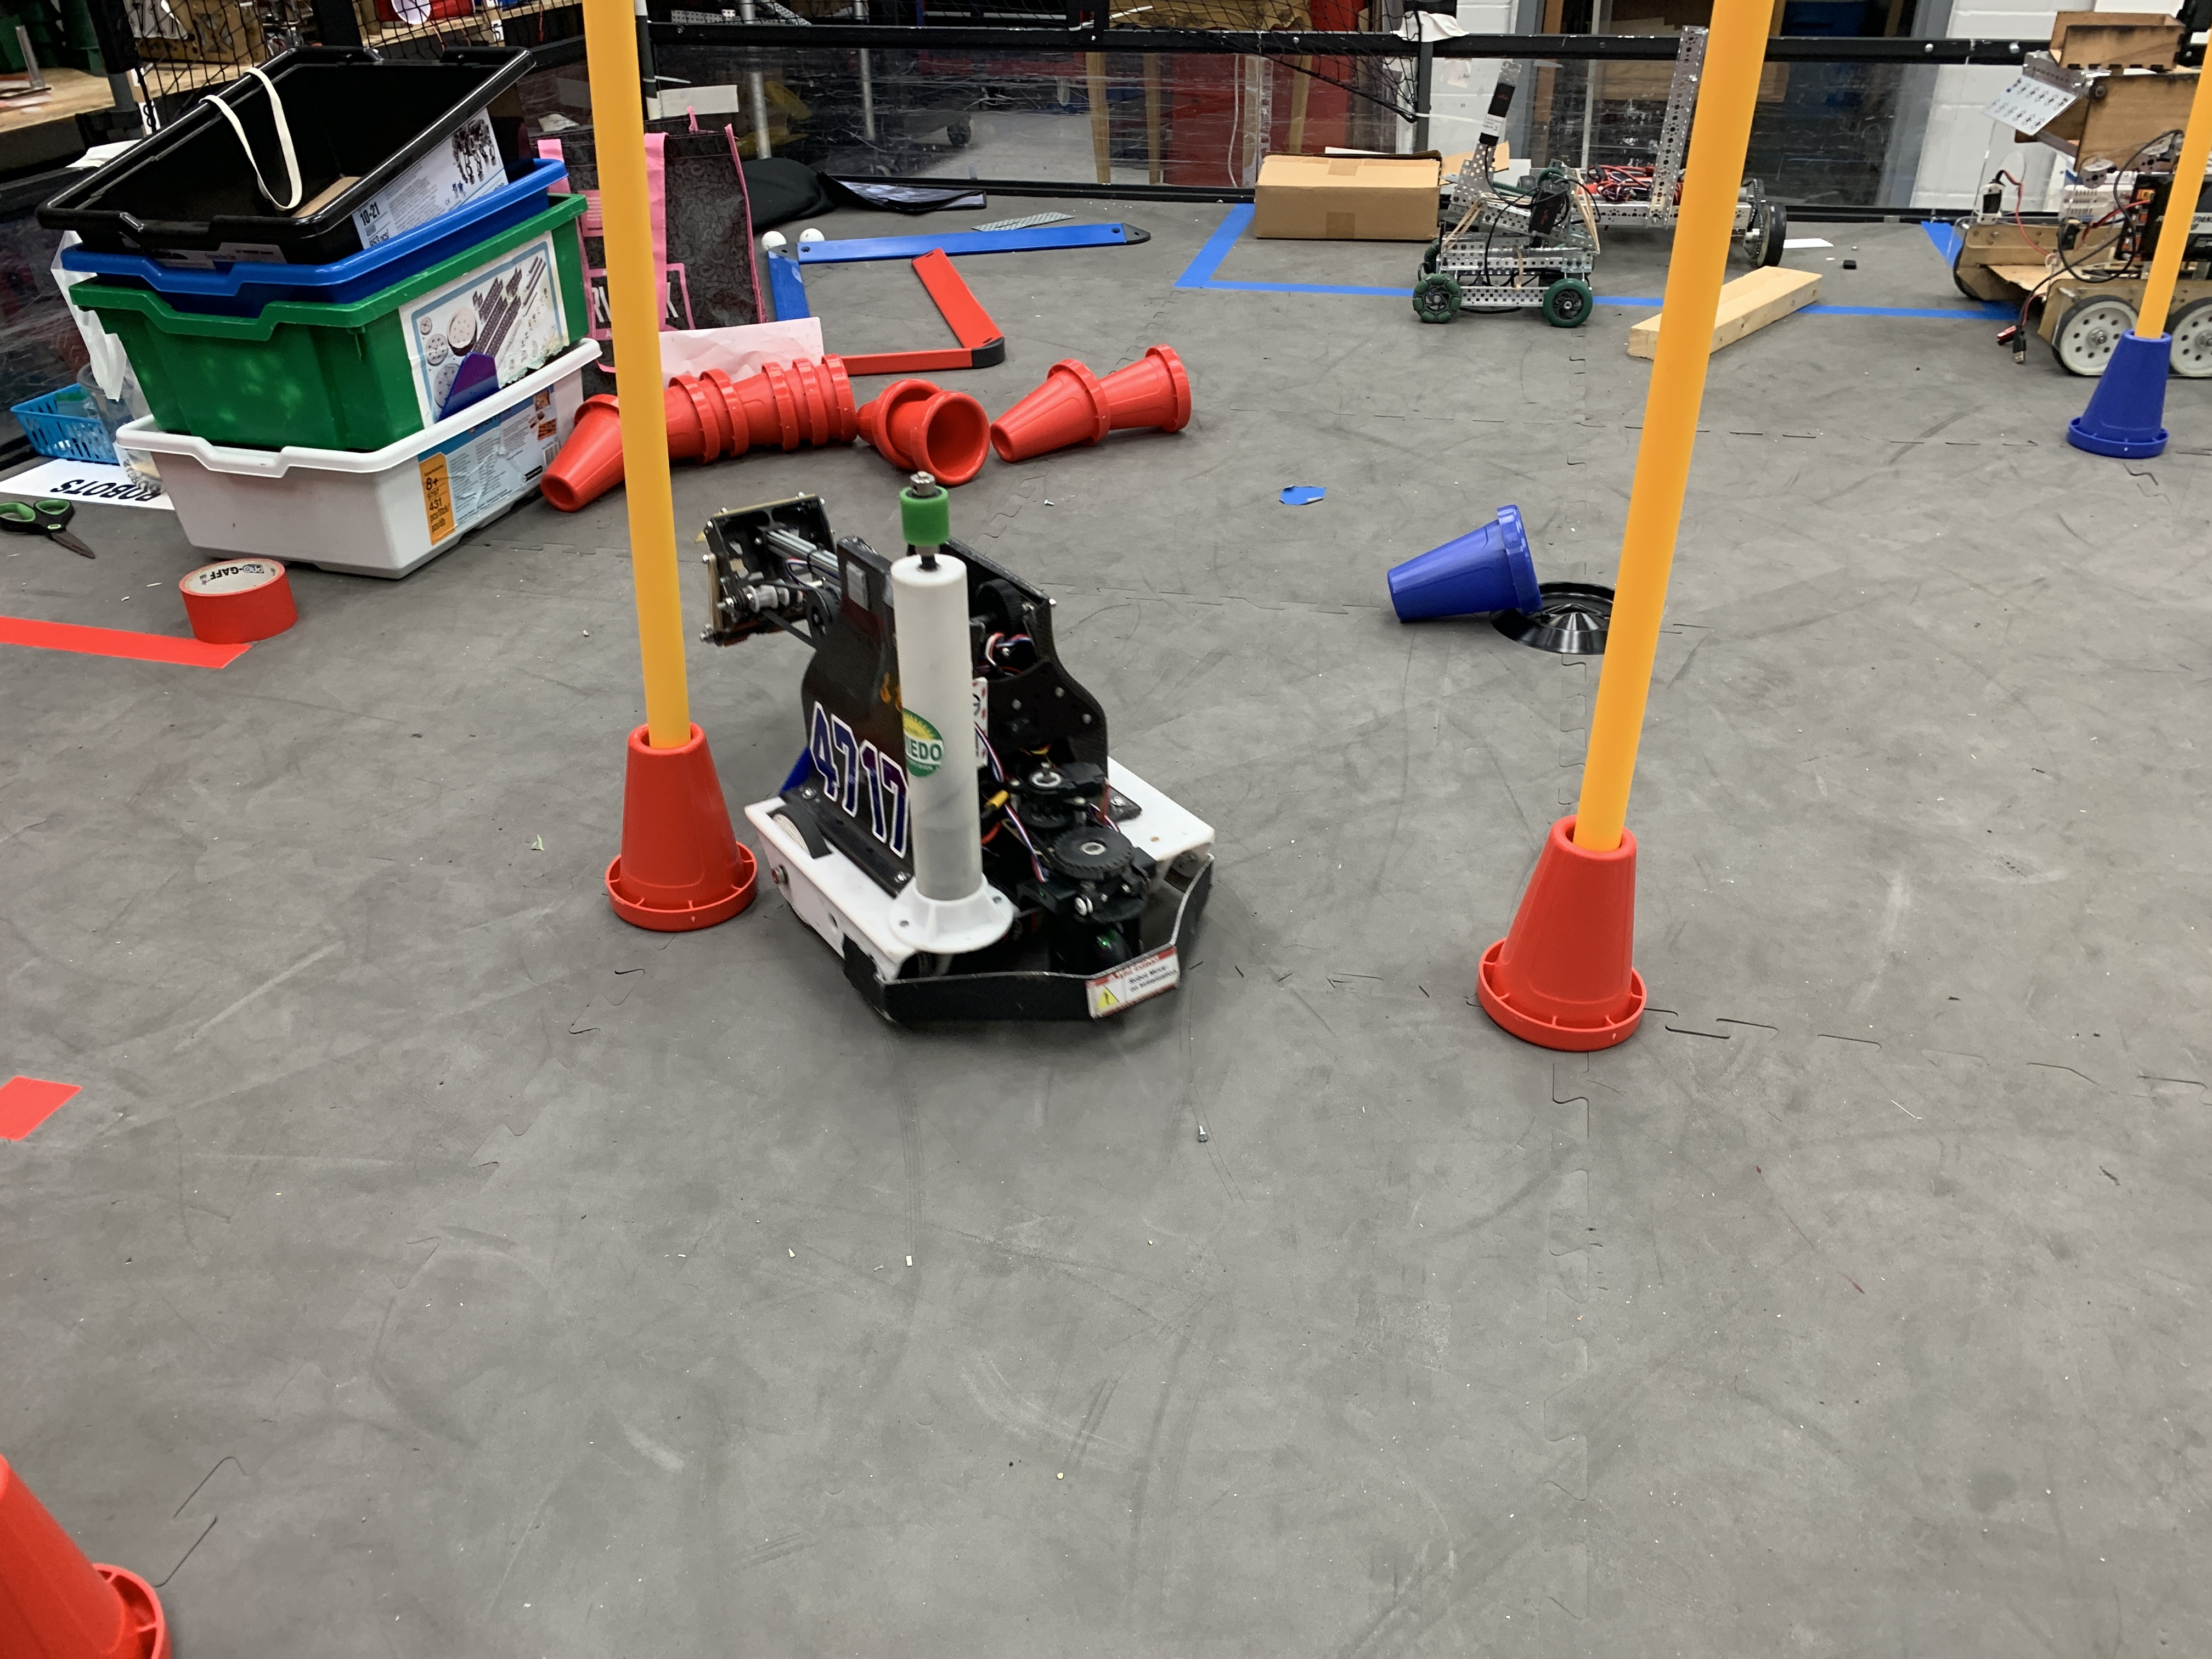
\includegraphics[width=0.95\textwidth]{Meetings/September/09-22-22/9-22-22_Hardware_Figure2.JPG}
  \caption{4717 robot from 2021-2022 season}
  \label{fig:pic2}
\end{minipage}
\end{figure}

\whatsnext{
\begin{itemize}
    \item Start researching and designing a tricycle drive design
    \item Start prototyping a mecanum drive
    \item Retest both options once both designs are fully constructed


\end{itemize} 
}
